\begin{figure}[!htbp]
\centering
\vspace{1\baselineskip}
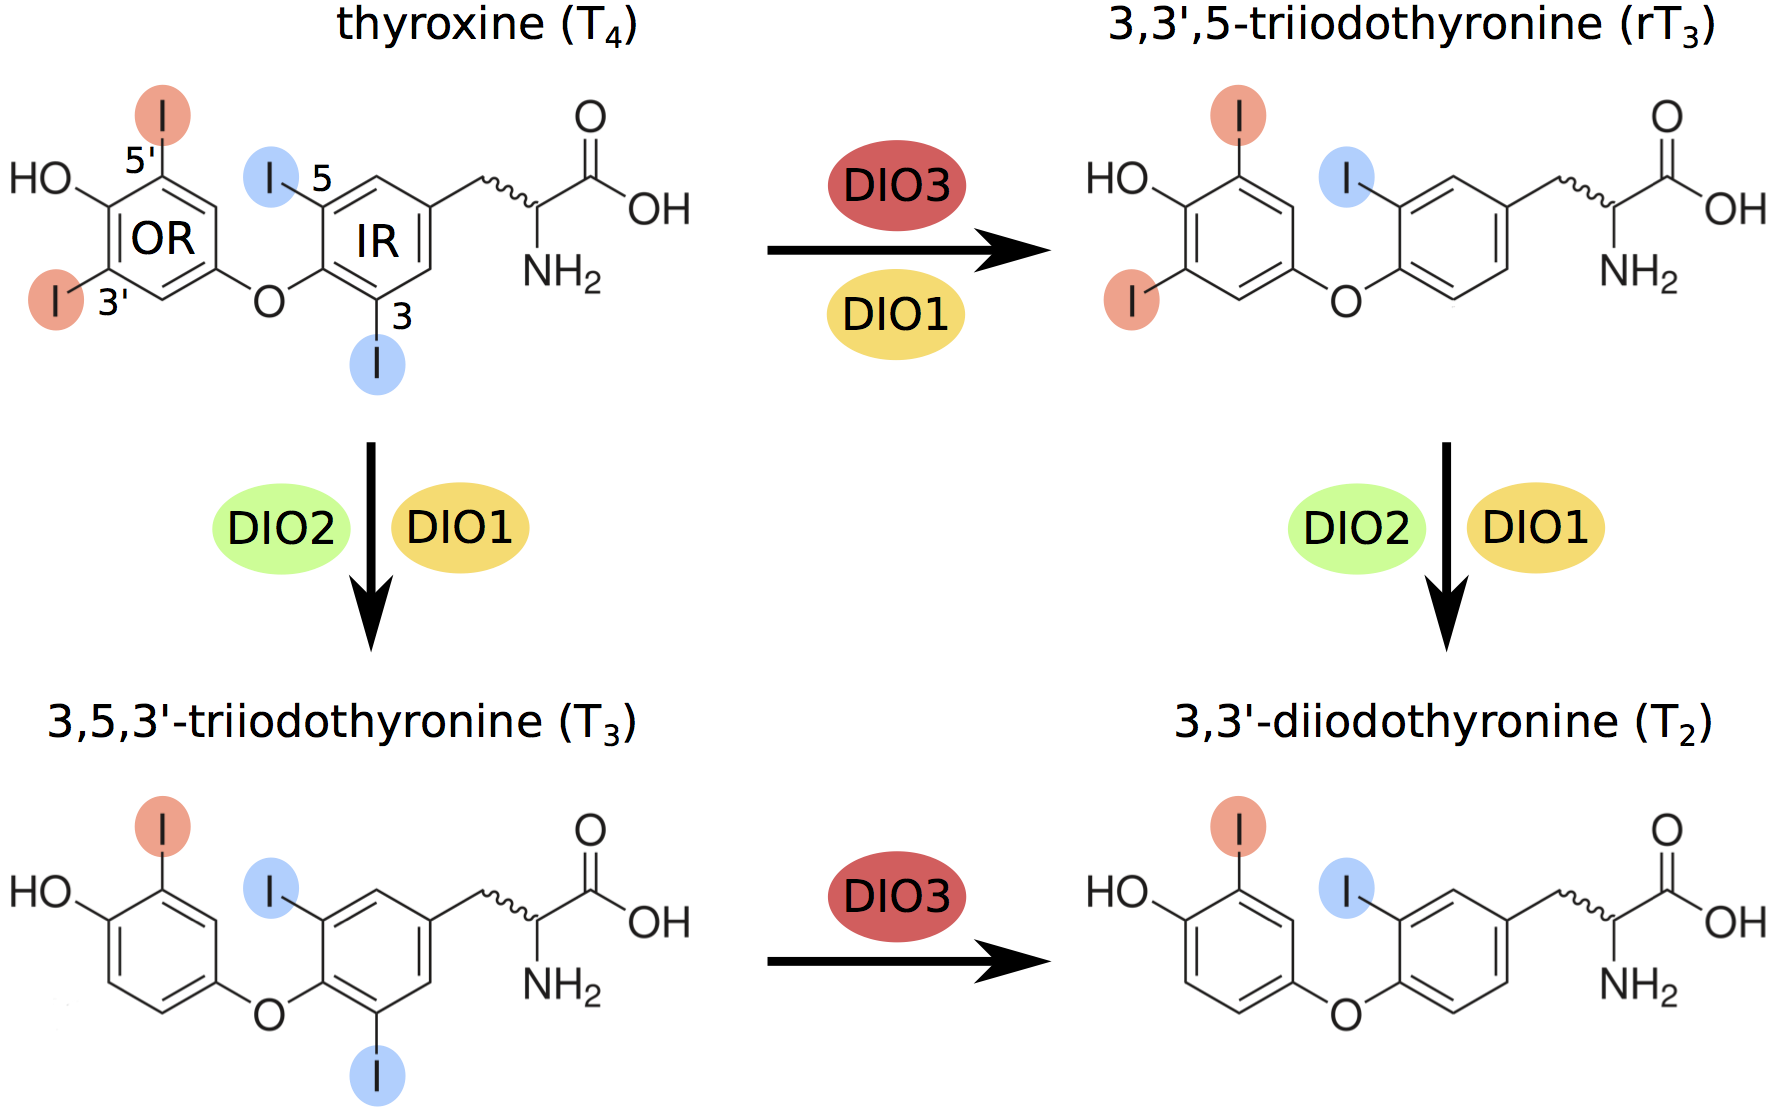
\includegraphics[width=\textwidth]
{Figures/ht-dio/ht-dio.png}
\caption[Réactions de désiodation de base]
{
Les réactions catalysées par les désiodases retirent les atomes d'iode (sphères rouges et bleues) du cycle externe (groupement phénol, positions 3' et 5', sphères rouges) ou du cycle interne (groupement tyrosine, positions 3 et 5, sphères bleues).
Ces voies peuvent activer la \gls{t4} en la transformant en \gls{t3} (\textit{via} \gls{dio1} ou \gls{dio2}) ou en l'empêchant d'être activée en la convertissant en la forme métaboliquement inactive \gls{rt3} (\textit{via} \gls{dio1} ou \gls{dio3}). La \gls{t2} est un produit commun aux deux voies, peu actif et rapidement métabolisé.
}
\label{fig:ht-dio}
\end{figure}